\begin{figure}[!htb]
\centering
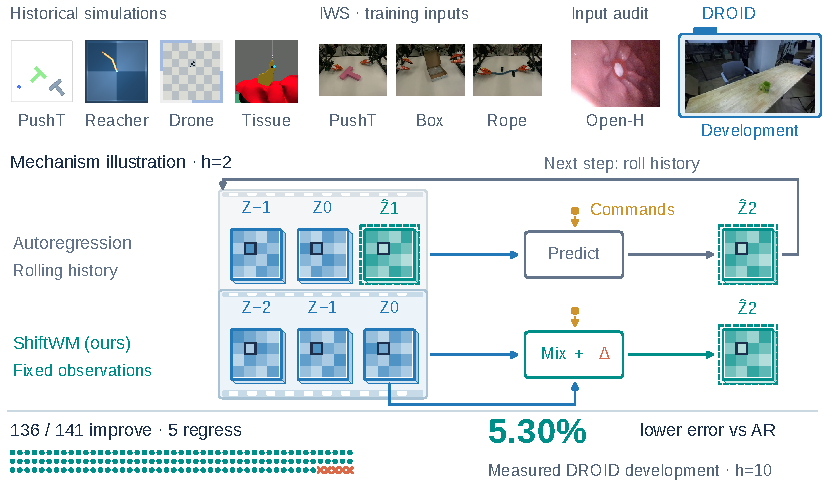
\includegraphics[width=\linewidth]{generated/editorial/teaser_visual_design.pdf}
\caption[Keep the observed feature history.]{\textbf{Keep the observed feature history.} The $h=2$ illustration contrasts autoregression, using $(Z_{-1},Z_0,\hat Z_1)$, with ShiftWM, retaining $(Z_{-2},Z_{-1},Z_0)$ and the fixed $Z_0$ decoder source. Autoregression inserts its own $\hat Z_2$ into the next window $(Z_0,\hat Z_1,\hat Z_2)$; its originally inferred support context remains fixed. Both receive the same available causal commands. Solid/dashed cards distinguish observed/predicted features; textures and outlined coordinates are schematic, not RGB predictions or measured feature values. Figure~\ref{fig:editorial-spatial-method} details the gated mixture and bounded correction. Gallery: historical simulations use distinct context models; IWS training is ongoing; Open-H is a physical-phantom input audit only. The measured footer retains all 141 DROID development episodes: 5.30\% lower population mean native, training-standardized $h=10$ feature MSE than matched autoregression (uncertainty in Figure~\ref{fig:editorial-spatial}). Images: DROID and Open-H (CC BY 4.0); IWS \citep{zhang2026rlawm}. Source-selection and simulator attribution accompany the editable figure.}
\label{fig:editorial-teaser}
\end{figure}
